\section{Magnetometer}\label{section:magnetometer}
The smartphone moves along the y-axis, but sometimes the phone rotates around the x- and z-axis when the player moves, which gives a smaller acceleration in the y-axis. 
To correct the accelerometer reading, the magnetometer can be used.
Using the magnetometer, the initial orientation can be found, which then can be compared to the current orientation to find the angle difference.
To find the orientation of the magnetometer, the phone was held in four different positions. 

Drawings of these positions can be seen in \figref{figure:magnetometer-headings}.
Each drawing and its corresponding caption, shows the geographical north pole and the heading of the smartphone.
\figref{figure:position-yz} illustrates how the phone should be held when the application is in use and the +z-axis is directed north. 
The magnetometer showed an angle of $270^\circ$, which is west, hereby, it could be concluded that the orientation of the magnetometer followed the -y-axis.
When the phone is tilted as seen in \figref{figure:position-xz} and \figref{figure:position-xy}, the y-axis was now in a vertical direction and the +z-axis was directed north, the magnetometer gave an angle of $0^\circ$ and $90\circ$, respectively. 
This angle indicated that when the y-axis is at a vertical direction the +z-axis becomes the direction in which the magnetometer measures its angle.\fxwarning{Det kan man ikk konkluderer udfra billederne, der mangler et forsøg hvor y peger nedad og z er vendt væk fra nord.}
\figref{figure:position-yx} were used to confirm that whenever the y-axis is in a horizontal direction, the -y-axis is the direction in which the magnetometer measures its angle.
When the different directions of the magnetometer are known, they can be used to correct the affected readings from the acceleration in the y-axis.

%Direction Hvilken vej noget vender/peger
%Heading er et resultat
%Orientaion hvordan telefonen er bygget/orienteret
%Allignment hvordan man står i forhold til noget

\begin{figure}[H]
	\centering
	%---- linebreak	
	\begin{subfigure}[b]{0.45\textwidth}
		\centering
		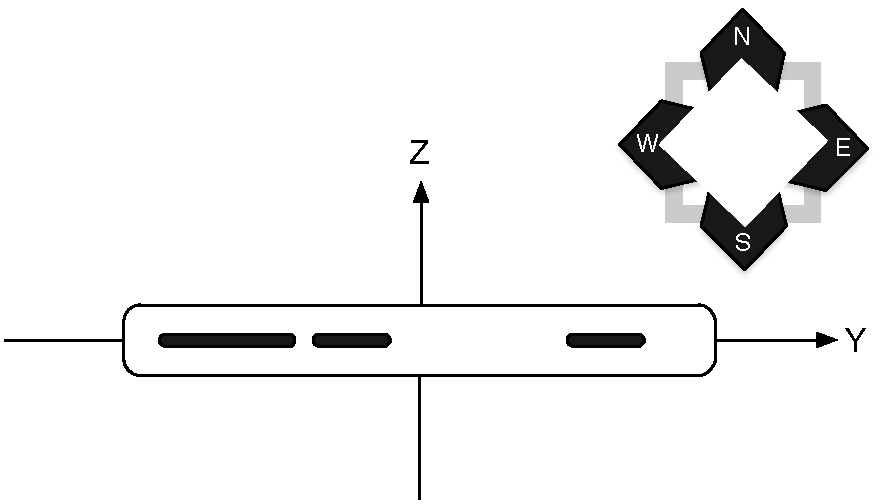
\includegraphics[scale = 0.4]{media/phone-rotation/phone-compass-a}
        \caption[caption]{The side of the phone.\\Magnetometer reading: $270^{\circ}$.}
		\label{figure:position-yz}
	\end{subfigure}
	\qquad
	\begin{subfigure}[b]{0.45\textwidth}
		\centering
		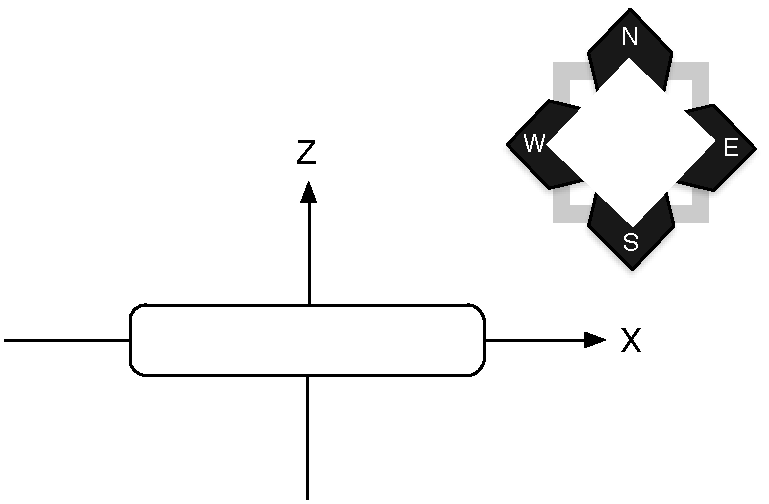
\includegraphics[scale = 0.4]{media/phone-rotation/phone-compass-b}
        \caption[caption]{The top of the phone.\\Magnetometer reading: $0^{\circ}$.}
		\label{figure:position-xz}
	\end{subfigure}
	%---- linebreak
	\begin{subfigure}[b]{0.45\textwidth}
		\centering
		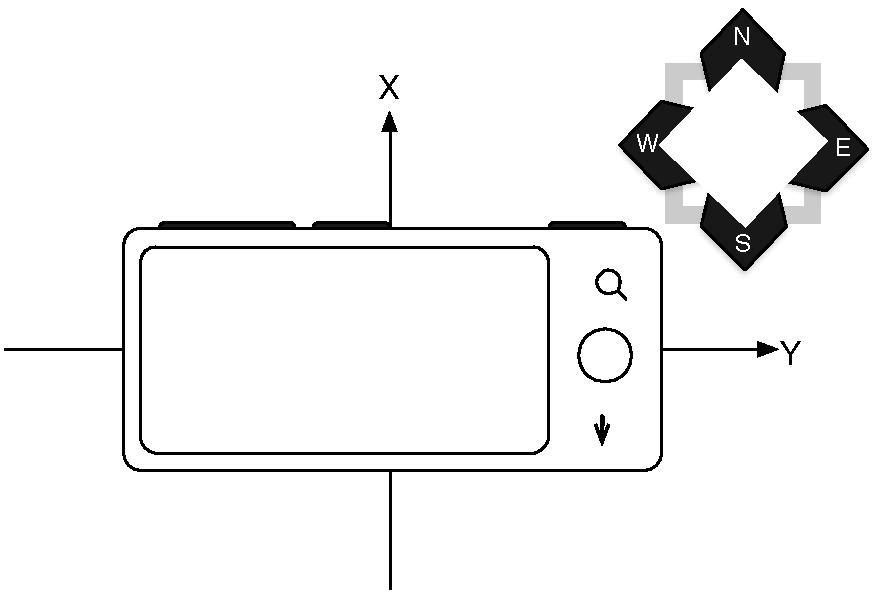
\includegraphics[scale = 0.4]{media/phone-rotation/phone-compass-c}
        \caption[caption]{The front of the phone, in landscape mode.\\Magnetometer reading: $270^{\circ}$.}
		\label{figure:position-yx}
	\end{subfigure}
	\qquad
	\begin{subfigure}[b]{0.45\textwidth}
		\centering
		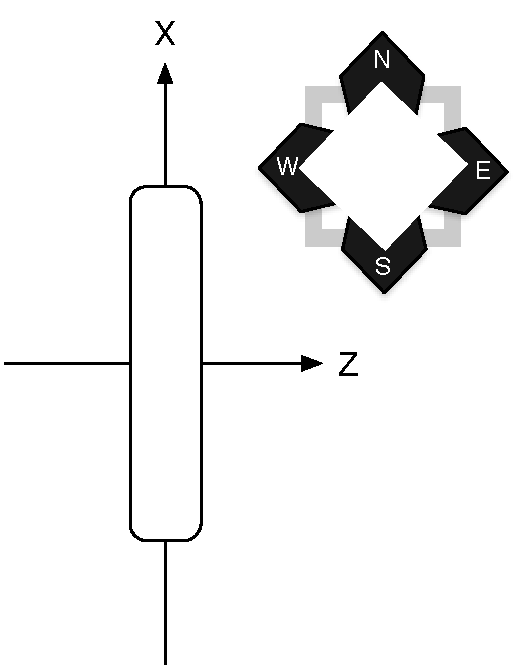
\includegraphics[scale = 0.4]{media/phone-rotation/phone-compass-e}
        \caption[caption]{The top of the phone.\\Magnetometer reading: $90^{\circ}$.}

		\label{figure:position-xy}
	\end{subfigure}		
	\caption{The orientation of the phone and its corresponding magnetometer reading. All drawings are seen from above.}
	\label{figure:magnetometer-headings}
\end{figure}
